\documentclass[lettersize,journal]{IEEEtran}
\usepackage{amsmath,amsfonts}
\usepackage{algorithmic}
\usepackage{array}
\usepackage[caption=false,font=normalsize,labelfont=sf,textfont=sf]{subfig}
\usepackage{textcomp}
\usepackage{stfloats}
\usepackage{url}
\usepackage{verbatim}
\usepackage{graphicx}
\hyphenation{op-tical net-works semi-conduc-tor IEEE-Xplore}
\def\BibTeX{{\rm B\kern-.05em{\sc i\kern-.025em b}\kern-.08em
    T\kern-.1667em\lower.7ex\hbox{E}\kern-.125emX}}
\usepackage{balance}
%\usepackage{natbib}
\usepackage{cite}
\usepackage{tabularx}
\hyphenpenalty=25
\tolerance=10000
\allowdisplaybreaks[4]
\usepackage{tcolorbox}
\newcommand{\ciao}[1]{{\setlength\fboxrule{0pt}\fbox{\tcbox[colframe=black,colback=white,shrink tight,boxrule=0.5pt,extrude by=1mm]{\small #1}}}}
% \usepackage{fontspec}
% \usepackage{libertine}

\setlength{\abovedisplayskip}{1ex}
\setlength{\belowdisplayskip}{1ex}

\usepackage[colorlinks=true,linkcolor=black,citecolor=blue,urlcolor=blue,]{hyperref}

\begin{document}
% \libertineGlyph{uni2460} \libertineGlyph{uni24F5} \libertineGlyph{uni2776}


\title{\vspace{-0.5cm}
%$H$-$D$ Support Set: Frequency Dynamic Security Analysis through Multidimensional Frequency Parameter Bindings
$H$-$D$ Support Set:  Identifying Frequency Dynamics by Constraining Multidimensional Frequency Parameter Bounds
}
\author{Yiping Yuan, Member, \textit{IEEE}, Liqian Zhu, Student Member, \textit{IEEE}, Zhenyuan Zhang, Senior Member, \textit{IEEE}, Weihao Hu, Senior Member, \textit{IEEE}, Zhe Chen, Fellow, \textit{IEEE}
}
\IEEEaftertitletext{\vspace{-2.5\baselineskip}}

\markboth{Journal of \LaTeX\ Class Files,~Vol.~18, No.~9, September~2020}%
{frequency dynamic identification through multi-dimensional frequency parameter bindings}

\maketitle


\begin{abstract}

  Existing research on the system frequency response (SFR) and frequency-oriented studies primarily relies on the commonly-used metrics such as  rate-of-frequency-change (RoCoF), nadir, and quasi-steady-state (Qss). Nevertheless, the complex interdependencies among these multidimensional frequency parameters have not been fully explored. This letter introduces a new criterion, termed as $H$-$D$ support set, to assess frequency stability by considering multidimensional relationships between these frequency parameters. An analytical solution is derived to quantify these interdependencies, and a convex polygon representation is constructed to visualize the feasible operating region defined by these parameters. Using this criterion, the impact of different frequency parameter configurations on system stability can be clearly obtained and analyzed. The effectiveness of the proposed approach is demonstrated on a modified IEEE 30-bus test system.

\end{abstract}

\begin{IEEEkeywords}
System frequency response, $H$-$D$ support set, multidimensional frequency parameters.
\end{IEEEkeywords}

\vspace{-0.25cm}

\section{Introduction}
\IEEEPARstart{T}{he} low inertia character of electrical power system significantly impact the system frequency security, which implicitly change the scheduling commitment results provided by different generators. In such circumstances, existing studies about power system dynamic response~\cite{8918440,10168982}, storage device sizing and control parameter tunning~\cite{markovic2019optimal}, optimal scheduling operation~\cite{9765359,10554988,10819485}, and  medium-term~\&~long-term generation planning studies~\cite{10820061,10938039}, trends to emphasis the consideration of frequency dynamic processes.


% The primary objective of frequency-oriented studies mentioned before is to determine the safety of frequency dynamic processes, as characterized by multidimensional frequency parameters such as inertia, damping and droop, reserves, etc. A conventional approach involves establishing dynamic frequency criteria, encompassing constraints on RoCoF, nadir, and QSS, typically expressed as mathematical relationships between these frequency parameters, to ensure frequency security. System stability is then assessed by evaluating whether the observed frequency dynamics remain within the feasible region defined by these criteria.  From this perspective, it is only possible to qualitatively assess whether the current configuration of frequency parameters is reasonable. However, it cannot refer the safety boundaries of multidimensional frequency parameters.

The primary objective of frequency-oriented studies as previously discussed is to ascertain the security of frequency dynamic, while it can be described through the SFR function, typically expressed by multidimensional frequency parameters, including system-level/regional-level $inertia$, $damping$, $droop$, and $reserve$, etc. Conventional methodologies establish dynamic frequency criteria, typically represented as mathematical constraints such as RoCoF, nadir and Qss~\cite{markovic2019optimal,8918440,10168982,9765359,10554988,10819485,10820061,10938039}. These criteria define a feasible operating region within which frequency dynamics are deemed secure~(see fig.~\ref{fig:sfr}). System stability is subsequently evaluated by determining if the frequency derivation derived from the SFR function remains within this defined region.

Nevertheless, these conventional approaches suffers from an implicitly limitation: it provides only a qualitative assessment of the current frequency parameter configuration's reasonableness. While it can determine if the system operates within predefined frequency dynamic thresholds, it fails to explicitly delineate the precise safety boundaries of these multidimensional frequency parameters. Consequently, it can neither directly quantify the margins of frequency safety, nor provide actionable insights into how to adjust these parameters to enhance system frequency security.

\begin{figure}[!t]
	\centering
	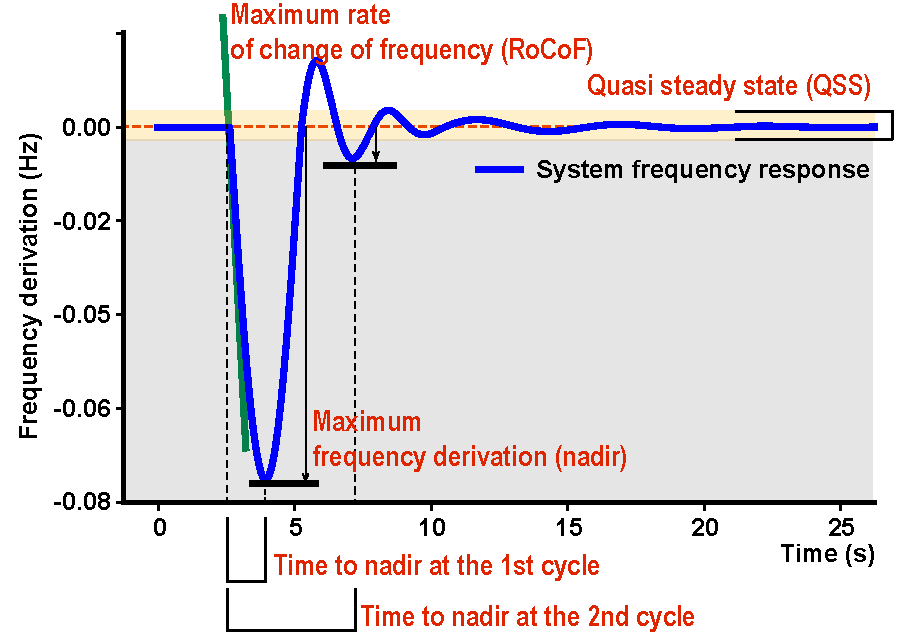
\includegraphics[width=0.4\textwidth,height=4.5cm]{frequency_response.pdf}\vspace{-0.25cm}
	\caption{The frequency dynamic process in the low inertia grid}\vspace{-0.25cm}
	\label{fig:sfr}
\end{figure}

This letter introduces a new criterion, termed as $H$-$D$ support set, to access the feasible bounds of multidimensional frequency parameters. Furthermore, an open-source tool (repository address: \url{https://github.com/Divas1234/frequencyregions.git}) for $H$-$D$ support set simulation is made freely available. Leveraging the SFR theorem, the interaction between multidimensional frequency parameters is analyzed, and both the upper and lower bounds of these parameters are explicitly estimated. In contrast to existing methodologies, the $H$-$D$ set provides a well-defined boundary interval for frequency parameters, thereby enabling more effective tuning optimization of frequency control parameters and facilitating comprehensive frequency security analysis.

\vspace{-0.25cm}
\section{SFR theorem in low inertia grid}

Given such a low inertia power system that considers high penetration of converters, the uniform analytical expression of frequency dynamic processes can be written as,

\vspace{-0.25cm}
\begin{subequations}
\begin{align}
  \!\!\!\!&\varDelta f(s) \!=\! \frac{1+sT}{2H_{EQU}T_{G}(s^2 + 2\zeta \omega_n s + \omega_n^2)}\frac{\varDelta P_{Step}}{s}\label{eq:Lsfr}\\
  \!\!\!\!&\omega_n \!=\! \sqrt{\!\frac{D_{EQU} \!+\! R_G}{2H_{EQU}T_G}}, \zeta \!=\! \frac{2H_{EQU}  \!+\! T_G(D_{EQU} \!+\! F_G)}{2\sqrt{2H_{EQU}T_G(D_{EQU} \!+\! R_G)}}
\end{align}
\end{subequations}

\noindent
where $\varDelta f(s)$ represents the frequency derivation with a step-type power disturbance $\varDelta P_{Step}$, $H_{EQU},\! D_{DEQ}$, respectively, describes the equivalent inertia parameter and damping parameter. $T_G$ is the time constant of conventional generator, $R_G$ denotes the aggregated droop parameter generated by conventional generators, $F_G$ denote the fraction of total power generated by high pressure turbines of conventional generators. In these formulations, the time constants within the transfer function of $\varDelta f(s)$ are normalized to unity, and the response times of converters with diverse control schemes are approximated as negligible. A more detailed feasibility analysis is provided in \cite{markovic2019optimal}.

In correlation with (1), the maximum frequency deviation, termed as $\max[ \varDelta f(t)]$, as well as the maximization rate of frequency change, termed as $\max[\varDelta f'(t)]$, can be derived~\cite{markovic2019optimal},

\vspace{-0.25cm}
\begin{subequations}
\begin{align}
    \max[\Delta f(t)] &= \varDelta f(t)|_{t=t_{nadir}^k} = -\frac{\Delta P_{Step}}{D_{EQU} + R_G} \bigg( 1 + \notag \\
                      &\left. (-1)^k \sqrt{\frac{T_G(R_G - F_G)}{2H_{EQU}}} e^{-\zeta \omega_n t_{nadir}^k} \right) \label{eq:max_delta_f}\\
    t_{nadir}^k &= \frac{1}{\omega_d} \arctan \left( \frac{\omega_d}{\zeta \omega_n - T_G^{-1}} \right) + \frac{k\pi}{\omega_d}\notag  \\
    \omega_d &= \omega_n \sqrt{1 - \zeta^2}, \quad \phi = \sin^{-1} \left( \sqrt{1 - \zeta^2} \right) \notag\\
  \max[\varDelta f'(t)] &= \varDelta f'(t)|_{t=t_{0}} = \frac{1}{2} H_{EQU}^{-1}\varDelta P_{Step} \label{eq:max_rocof}\\
  \varDelta f_{QSS}(t) &= \varDelta f(t)|_{t=t_{\infty}} = {D_{EQU}^{-1}\varDelta P_{Step}} \label{eq:qss}
\end{align}
\end{subequations}

\noindent
where $\max [\varDelta f(t)]^k$ enforces the maximum frequency deviation at the $k$-th cycle, $\max [\varDelta f'(t)]$ defines the maximum rate of change of frequency derivation, $\varDelta f_{QSS} (t)$ denotes the (quasi) steady-state frequency deviation, $t_{nadir}^k$ denotes the time to the $k$-th nadir of the frequency deviation.


To ensure the security of frequency dynamics across the entire frequency response processes, the amounts of $\max[\varDelta f(t)]$, $\max[\varDelta f'(t)]$ and $\varDelta f_{QSS}(t)$ must be constrained within the predefined frequency dynamic restrictions, as discussed in existing frequency-oriented studies~\cite{9765359,10554988,10819485,10820061,10938039},

\vspace{-0.25cm}
\begin{subequations}
  \begin{align}
  \left \{
  \begin{array}{rr}
  {Nadir\,\, constraint:}& \max[\varDelta f (t)] \leq \gamma_{Nadir}\\
  {RoCoF\,\, constraint:}&\max[\varDelta f' (t)] \leq \gamma_{RoCoF}\\
  {QSS\,\, constraint:} &\varDelta f_{QSS} (t) \leq \gamma_{QSS}\\
\end{array}
\right.
    \end{align}
  \end{subequations}

  \noindent
where $\gamma_{Nadir}$, $\gamma_{RoCoF}$ and $\gamma_{QSS}$ are predefined frequency dynamic restrictions concerning frequency nadir, RoCoF, and Qss frequency derivation, respectively.

\section{$H$-$D$ support set: A new criterion for frequency security identification}

This section derives explicit bounds of multidimensional frequency parameters, including inertia, damping, and droop gains, these bindings result in a new criterion for frequency security identification that differs from (3a).

The sufficient condition for the occurrence of maximum frequency derivation (nadir) is predicated on the convergence of the transfer function (1a) and the non-negativity characteristic of time-to-nadir coefficient. For the first category, this translates to the mathematical requirement that all poles, as derived from the denominator of (1a), must lie within the left half of the complex $s$-plane. Since the amount of poles in (1a) can be written as $-\zeta \omega_n \pm \omega_n \sqrt{1 - \zeta^2}$, $\zeta \geq 0$ must hold to ensure the convergence of the transfer function. For the latter category, the amount of denominator should be positive to guarantee the non-negativity of time-to-nadir coefficient, that is, $\zeta \omega_n - T_G^{-1}\geq 0, \text{and}\, \sqrt{1-\zeta^2} \geq 0$. So, the determination conditions for the intermediate variables, $\zeta, \omega_n$, can be obtained,

\vspace{-0.25cm}
\begin{subequations}
  \begin{align}
    0 \leq \zeta \leq 1, \quad \zeta \omega_n \geq {T_G^{-1}} \label{eq:zeta_wn}
    \end{align}
  \end{subequations}

Substituting (1b) into (4a), the bounds of inertia and damping parameters can be further derived as below,

\vspace{-0.25cm}
\begin{subequations}
  \begin{align}
    H_{EQU} &\leq \frac{1}{2}T_G \left(\text{term}_1 + \sqrt{\text{term}_2} \right) \\
    H_{EQU} &\geq \frac{1}{2}T_G \left(\text{term}_1 - \sqrt{\text{term}_2} \right) \\
    H_{EQU} &\leq \frac{1}{2} (D_{EQU} + F_G) T_{G} \\
    \text{term}_1 &= (D_{EQU} - F_G + 2R_G) \\
    \text{term}_2 &= {(D_{EQU} - F_G + 2R_G)^2 - (D_{EQU} + F_G)^2}\\
    \text{term}_2 &\geq 0 \Longrightarrow (R_G - F_G)(R_G + D_{EQU}) \geq 0
    \end{align}
  \end{subequations}

Let $H_{EQU}=\mathcal{Q} (D_{EQU})$, the relationship between $H_{EQU}$ and $D_{EQU}$ can be constructed,

\vspace{-0.25cm}
\begin{subequations}
  \begin{align}
    \overbrace{\begin{array}{l}\frac{1}{2}T_G \left(\text{term}_1 - \sqrt{\text{term}_2} \right)\end{array}}^{lower\,bound} \leq H_{EQU}=\mathcal{Q} (D_{EQU}) \leq \notag \\
    \underbrace{\min \left [
    \begin{array}{l}
      \frac{1}{2}T_G \left(\text{term}_1 + \sqrt{\text{term}_2}\right), \frac{1}{2} (D_{EQU} + F_G) T_{G}\\
    \end{array} \right ]
    }_{upper\, bound}
    \end{align}
  \end{subequations}

Next, other relations between $H_{EQU}$ and $D_{EQU}$ concerning nadir, RoCoF, and Qss, can be extended from (3a). For simplification, let $\max [ \varDelta f(t)]=\mathcal{R} (H_{EQU}, D_{EQU})$ denotes the non-linear close form of (2a), then, more bindings between $H_{EQU}$ and $D_{EQU}$ can be found,

\vspace{-0.25cm}
\begin{subequations}
  \begin{align}
H_{EQU} &\!\geq\! \underbrace{\max\!\!\! \begin{array}{l}[\frac{1}{2} \gamma_{RoCoF}^{-1} \varDelta P_{Step},\mathcal{R}^{-1}(D_{EQU}) \gamma_{Nadir}]\end{array}}_{lower\, bound} \\
D_{EQU} & \geq \gamma_{QSS}^{-1} \varDelta P_{Step}
  \end{align}
\end{subequations}

% \textcircled{\small{2}}
By meticulously re-organizing the preceding derivations, a concise bounds for system inertia and damping parameters can be estimated from (6) and (7).

\vspace{-0.25cm}
\begin{subequations}
  \begin{align}
    \!\!\!\begin{array}{rl}
    \text{Inertia}\,\, \ciao{1}\, lower\,bound:&\!\!\!\frac{1}{2} \gamma_{RoCoF}^{-1} \varDelta P_{Step}\\
    \ciao{2}\,lower\,bound:&\!\!\!\frac{1}{2}T_G \left(\text{term}_1 - \sqrt{\text{term}_2} \right)\\
    \ciao{3}\,lower\,bound:&\!\!\!\mathcal{R}^{-1}(D_{EQU}) \gamma_{Nadir} \\
    \ciao{4}\,upper\,bound:&\!\!\!\frac{1}{2}T_G \left(\text{term}_1 + \sqrt{\text{term}_2} \right)\\
    \ciao{5}\,upper\,bound:&\!\!\! \frac{1}{2}(D_{EQU} + F_G) T_G\\
   \text{ Damping} \,\,\ciao{6}\,lower\,bound:&\!\!\! \gamma_{QSS}^{-1} \varDelta P_{Step}\\
    \end{array}
  \end{align}
\end{subequations}

\section{Case Studies and analysis}

A IEEE $30$ bus test system with two wind farms is applied to demonstrate the effectiveness of the proposed criterion. Both multidimensional frequency parameters provided by conventional generators and converters is sorted out in table~\ref{tab:generator_parameters}.

\vspace{-0.25cm}
\begin{table}[!h]
  \centering
  \caption{multidimensional frequency parameter configurations}\vspace{-0.25cm}
  \begin{tabular}{p{0.285\linewidth} p{0.1\linewidth} p{0.1\linewidth} p{0.1\linewidth} p{0.1\linewidth} p{0.05\linewidth}}
      \hline
      \textbf{Type} & $H$ [p.u.] & $D$ [p.u.] & $R$ [p.u.] & $F$ [p.u.] & $T$ [s] \\
      \hline
      \!\!\scriptsize{OCGT} & 6.0 & 0.6 & 0.05 & 0.35 & 8.0 \\
      \!\!\scriptsize{Converter (Virtual Inertia)} & 6.0 & 0.6 & - & - & - \\
      \!\!\scriptsize{Converter (Droop)} & - & - & 0.01 & - & - \\
      \hline
  \end{tabular}
  \label{tab:generator_parameters}
\end{table}
\vspace{-0.25cm}

It can be observed that the $H$-$D$ support set in fig.~\ref{fig:inertia_damping_supportset} formed by (8a) is an approximate convex polyhedron. In the aforementioned former five bounds in (8a) concerning inertia parameters, $\ciao{2}$ and $\ciao{4}$ represent redundant constraints, whereas $\ciao{1},\,\ciao{3},$ and $\ciao{5}$ are active constraint that restrict the actual feasible area of the $H$-$D$ set.
Remarkably, the RoCoF constraint termed as $\ciao{1}$, nadir constraint termed as $\ciao{3}$, and Qss constraint termed as $\ciao{6}$ are commonly-used frequency dynamic requirements, these constraints in frequency-oriented studies are also the main types of constraints that play a role in the constructions of $H$-$D$ support set, demonstrating the feasibility of $H$-$D$ support set in this work.

\begin{figure}[!t]\vspace{-0.125cm}
  \centering
  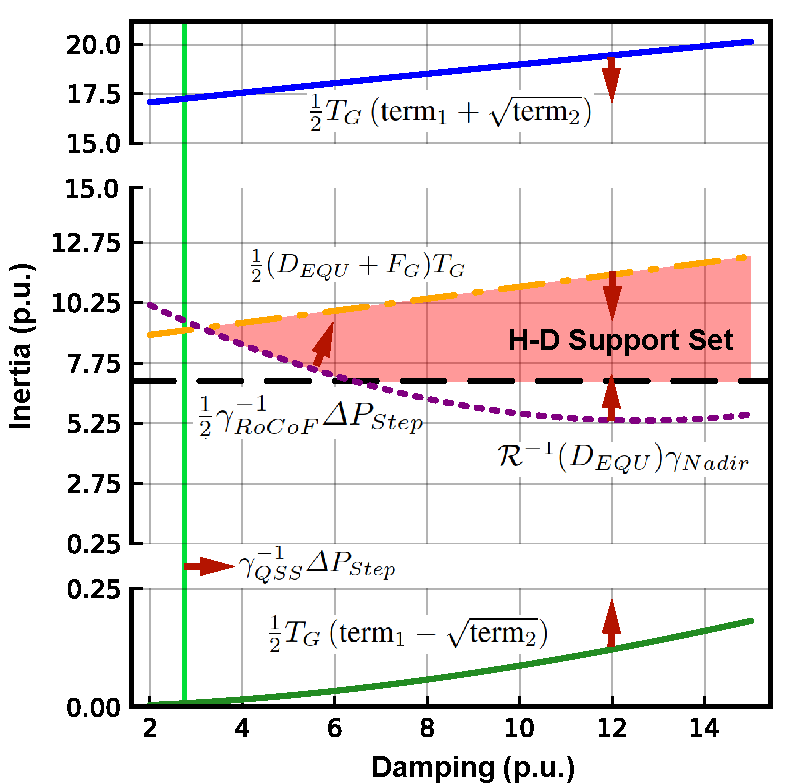
\includegraphics[width=0.4\textwidth,height=6.50cm]{inertia_damping_supportset.pdf}\vspace{-0.125cm}
  \caption{The feasible area of the $H$-$D$ support set in the low inertia system}\vspace{-0.25cm}
  \label{fig:inertia_damping_supportset}
\end{figure}

The difference from previous studies lies in that this letter additionally identifies more bounding conditions, and these refined bounding conditions, along with the addition of RoCoF, nadir, and Qss constraints, form a relatively closed polyhedron region.  In Fig.~\ref{fig:inertia_damping_supportset}, the scale of the $H$-$D$ set intuitively demonstrates the feasible range of multidimensional frequency  parameters. By specifically increasing the upper bound of inertia $H_{EQU}$, termed as $\ciao{5}$, the range of the $H$-$D$ set can be further expanded. Nevertheless, the upper bound of $H_{EQU}$ can be indirectly achieved by increasing the amount of equivalent damping parameter $D_{EQU}$.

\vspace{-0.25cm}

\begin{figure}[!h]
  \centering
  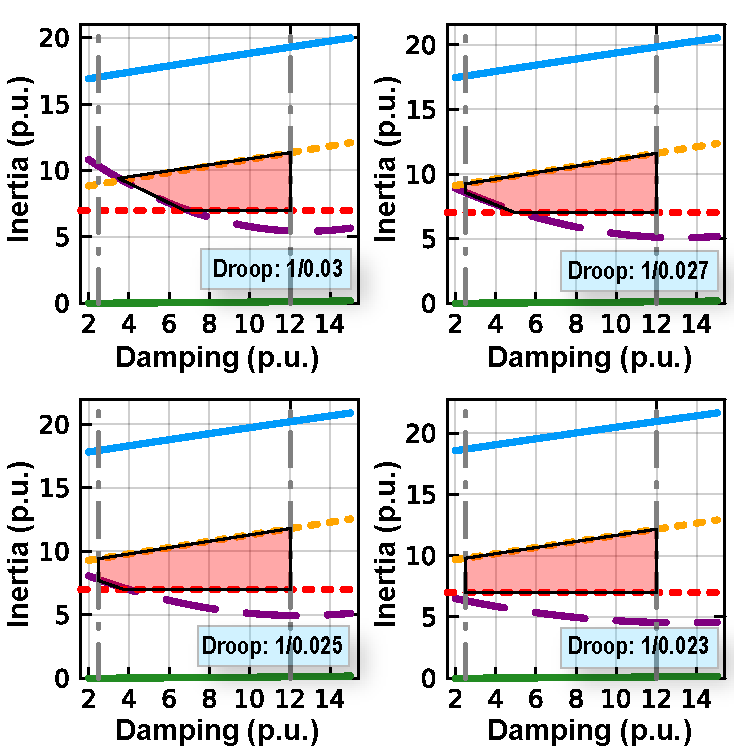
\includegraphics[width=0.425\textwidth,height=6.5cm]{inertia_damping_feasible_region.pdf}\vspace{-0.125cm}
  \caption{The variation in the extent of the $H$-$D$ support set across different frequency droop parameter configurations}\vspace{-0.25cm}
  \label{fig:inertia_damping_feasible_region}
\end{figure}

Moreover, the scope of $H$-$D$ support sets exhibits variation contingent upon droop parameter settings. However, once the droop gain surpasses a threshold of $1/0.023$, the $H$-$D$ set becomes invariant (see Fig.~\ref{fig:inertia_damping_feasible_region}), and it is exclusively determined by the inertia bounds $\ciao{1}$ and $\ciao{3}$. Fig.~\ref{fig:diff_inertia_damping_supportset} records the geometric characteristic of these $H$-$D$ sets under different multidimensional frequency parameter configurations.

\begin{figure}[!t]
	\centering
	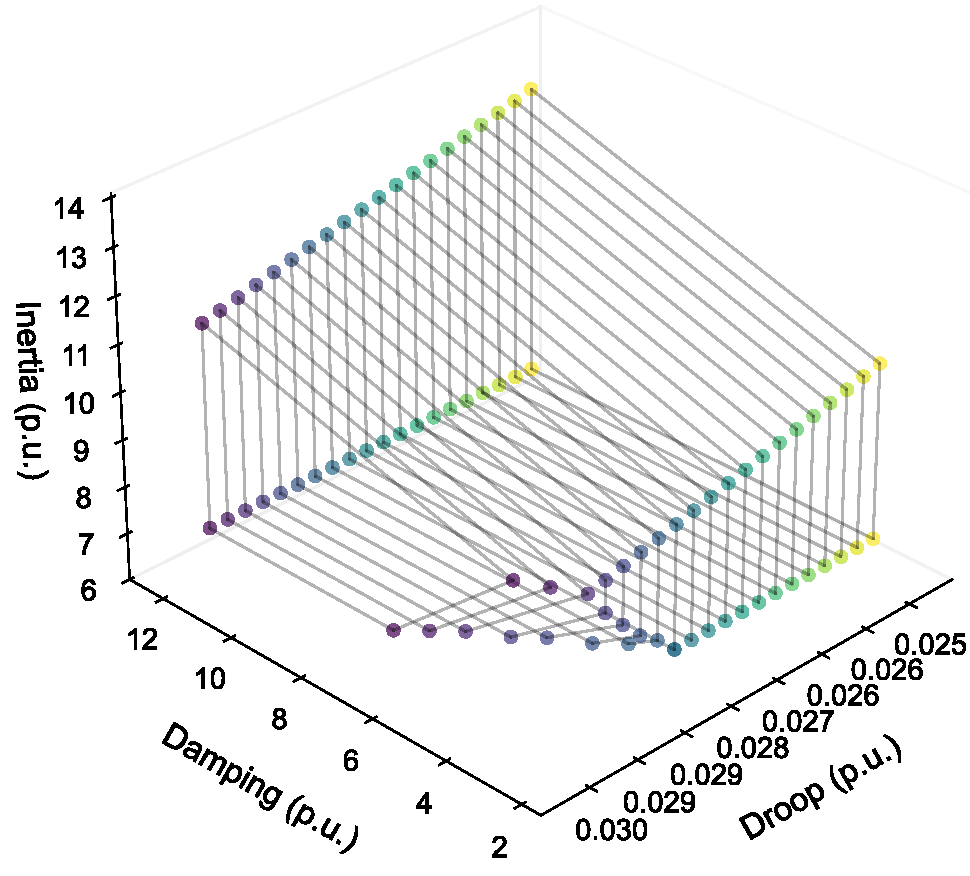
\includegraphics[width=0.305\textwidth,height = 5.5cm]{diff_inertia_damping_supportset.pdf}\vspace{-0.25cm}
	\caption{The geometric structure defined by the ensemble of $H$-$D$ sets across various multidimensional frequency parameter configurations}\vspace{-0.25cm}
	\label{fig:diff_inertia_damping_supportset}
\end{figure}


This observation highlights that for a public grid characterized by a comparatively low droop parameter (indicative of a relatively high frequency adjustment capability), further augmentation of system droop performance will not progressively expand the feasible operating region of the $H$-$D$ set. Instead, it becomes imperative to enhance the frequency safety margin by increasing system inertia and damping. In conjunction with the preceding analysis, $H$-$D$ support set offers more precise and intuitive recommendations for frequency parameters tuning and system operation optimization.


\section{Conclusion}

This letter details an analytical solution of multidimensional frequency bounds and introduces a new criterion, termed the $H$-$D$ support set, to characterize the feasible range of frequency parameters in low inertia grids. Furthermore, the polyhedral extent of $H$-$D$ support set is comparatively assessed across various frequency parameter configurations. The proposed methodology facilitates a clear visualization and comparative evaluation of the impact of different frequency parameters on the operating interval of the system, thereby serving as a guideline for ensuring that the system remains within its inherent feasible range.

%\section{References}
\bibliographystyle{IEEEtran}
\bibliography{IEEEabrv,reference}

\end{document}


